\documentclass[border=6pt]{standalone}
\usepackage{amsmath}
\usepackage{tikz}
\usetikzlibrary{arrows.meta}
\begin{document}
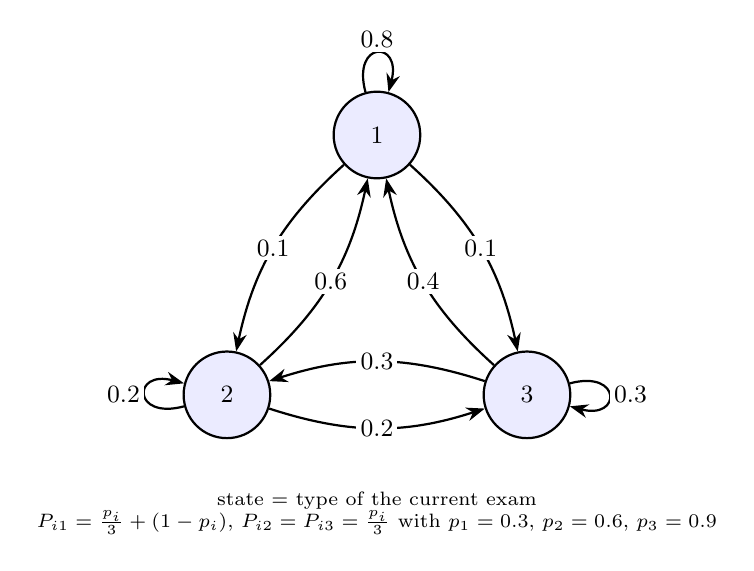
\begin{tikzpicture}[>=Stealth,font=\small,
 s/.style={draw,thick,circle,minimum size=1.1cm,inner sep=0pt,fill=blue!8},
 e/.style={->,thick},
 lab/.style={font=\small,fill=white,inner sep=1.5pt},
 every loop/.style={->,thick,looseness=6}]
\node[s] (1) at (90:2.2) {1};
\node[s] (2) at (210:2.2) {2};
\node[s] (3) at (-30:2.2) {3};
\draw[e] (1) to[bend right=18] node[lab]{0.1} (2);
\draw[e] (2) to[bend right=18] node[lab]{0.6} (1);
\draw[e] (1) to[bend left=18] node[lab]{0.1} (3);
\draw[e] (3) to[bend left=18] node[lab]{0.4} (1);
\draw[e] (2) to[bend right=18] node[lab]{0.2} (3);
\draw[e] (3) to[bend right=18] node[lab]{0.3} (2);
\path (1) edge[loop above] node[lab]{0.8} (1);
\path (2) edge[loop left] node[lab]{0.2} (2);
\path (3) edge[loop right] node[lab]{0.3} (3);
\node[font=\scriptsize,align=center] at (0,-2.6) {state = type of the current exam\\$P_{i1}=\tfrac{p_i}{3}+(1-p_i)$, $P_{i2}=P_{i3}=\tfrac{p_i}{3}$ with $p_1=0.3$, $p_2=0.6$, $p_3=0.9$};
\end{tikzpicture}
\end{document}
